\documentclass[
    11pt,
    a4paper,
    egregdoesnotlikesansseriftitles,
    toc=chapterentrywithdots,
    twoside,openright,
    titlepage,
    parskip=half,
    headings=normal,  % reduces heading size
    listof=totoc,
    bibliography=totoc,
    index=totoc,
    captions=tableheading,  % caption below table
    chapterprefix,
    listof=flat,
    final
]{scrbook}


% details about your thesis
\newcommand{\titel}{Transformer}
\newcommand{\artderarbeit}{Projektentwurf}  % {Bachelorarbeit,Masterarbeit}
\newcommand{\autor}{Sarah Volkamer}
\newcommand{\studiengang}{Angewandte Mathematik und Physik}  

% custom head and foot

\usepackage[automark]{scrlayer-scrpage}
\pagestyle{scrheadings}
%\ihead{\headmark}
\chead{}
%\ohead{\pagemark}
\renewcommand*\chaptermarkformat{\chapappifchapterprefix{\ }% 
  \thechapter.\enskip}

\RedeclareSectionCommand[tocindent=0pt]{section}
\RedeclareSectionCommand[tocindent=0pt]{subsection}
%\RedeclareSectionCommand[tocnumwidth=70pt]{chapter}


% other packages
\usepackage{minted}
\usepackage[utf8]{inputenc}
\usepackage[T1]{fontenc}
\usepackage{lmodern,relsize,textcomp,csquotes}
\usepackage{amsmath,amsfonts}
\usepackage[english,ngerman]{babel}  % flip for German thesis
\usepackage[final]{graphicx}
\usepackage{setspace,geometry,xcolor}
\usepackage{makeidx}
\usepackage{paralist,ifthen}
\newcommand{\todo}[1]{}
%\usepackage{todonotes}
\usepackage{url}
\usepackage[toc]{glossaries}
\usepackage{pdfpages}
\usepackage{acronym}
\usepackage[most]{tcolorbox}
\usepackage{upgreek}
\usepackage{xcolor}
\usepackage{mathtools}
\usepackage{textpos}
\usepackage{varwidth}
\usepackage{svg}

\tcbuselibrary{listings}
\tcbset{listing engine=listings}
\definecolor{codecomments}{rgb}{0,0.6,0}
\definecolor{codekeywords}{rgb}{0, 0, 0.75}
\definecolor{codestrings}{rgb}{0.75, 0.25, 0}
\definecolor{codebgcolor}{rgb}{0.95,0.95,0.95}


\usepackage{varioref}
\usepackage{float}

% table setup
\usepackage{longtable}
\usepackage{colortbl}
\usepackage{booktabs}
\usepackage{array}
\usepackage{ragged2e}
\usepackage{lscape}
\usepackage{multirow}
\usepackage[backend=biber]{biblatex}
\addbibresource{Quellen.bib}

% pdf hyperref
\usepackage[
    bookmarks=true,
    bookmarksopen=true,
    bookmarksnumbered=true,
    bookmarksopenlevel=1,
    pdftitle={\titel},
    pdfauthor={\autor},
    pdfcreator={\autor},
    pdfsubject={\titel},
    pdfkeywords={\keywords},
    pdfpagelabels=true,
    colorlinks=true,
    linkcolor=red,
    urlcolor=magenta,
    anchorcolor=black,
    citecolor=cyan,
    filecolor=magenta,
    menucolor=red,
    plainpages=false,
    hypertexnames=true,
    linktocpage=true,
\left( ]{hyperref}
\usepackage[ngerman]{cleveref}


\usepackage{scrhack}
% configure your listings style
\usepackage{listings}
\lstset{
	tabsize=3,
	extendedchars=true,
	frame=single,
	showstringspaces=true,
	numbers=left,
	numberstyle=\small,
	breakautoindent=true,
	mathescape=true
}

% page setup
%\setlength{\topskip}{\ht\strutbox}
\geometry{paper=a4paper,left=2.5cm,top=3.0cm,bindingoffset=.8cm}
\onehalfspacing
\frenchspacing
\clubpenalty = 10000
\widowpenalty = 10000 
\displaywidowpenalty = 10000
\raggedbottom % Text soll nicht über die gesamte Seite verteilt sein

% some commands
\newcommand{\ua}{\mbox{u.\,a.\ }}
\newcommand{\zB}{\mbox{z.\,B.\ }}
\newcommand{\dahe}{\mbox{d.\,h.,\ }}
\newcommand{\bzw}{\mbox{bzw.\ }}
\newcommand{\bzgl}{\mbox{bzgl.\ }}
\newcommand{\eg}{\mbox{e.\,g.\ }}
\newcommand{\ie}{\mbox{i.\,e.\ }}
\newcommand{\wrt}{\mbox{w.\,r.\,t.\ }}
\newcommand{\etal}{\mbox{\emph{et.\,al.\ }}}


% TODO remove if not needed...
\usepackage{blindtext}
\usepackage{fontawesome5}

% load glossary entries
%\makenoidxglossaries
%\loadglsentries{glossary}

\newtcolorbox[auto counter, 
crefname={Definition}{Definitionen}]%
{definition}[1][]{arc=0mm,
	colback=white,
	coltitle=black,
	colframe=red!40!white,
	fonttitle=\sffamily,
	code={\def\mytitle{#1}},
	title=Definition \thetcbcounter, #1
}

\newtcblisting{python}{left = 2mm, right = 0mm, colback=white, colframe=white, listing only, listing options = 
	{
		language=Python,
		numbers=left, 
		backgroundcolor=\color{codebgcolor},
		numberstyle=\small\color{red!75!black}, commentstyle=\color{codecomments},
		keywordstyle=\bfseries\color{codekeywords},
		stringstyle=\color{codestrings}
	}
}
\newtcblisting{pythonzwei}{breakable, left = 1mm, right = 0mm, colback=white, colframe=white, listing only, listing options = 
	{
		language=Python,
		gobble=4,
		numbers=left, 
		backgroundcolor=\color{codebgcolor},
		numberstyle=\small\color{red!75!black}, commentstyle=\color{codecomments},
		keywordstyle=\bfseries\color{codekeywords},
		stringstyle=\color{codestrings}
	}
}

\begin{document}
\include{content/definitions}

\setcounter{secnumdepth}{3}  % numerate subsections
\setcounter{tocdepth}{2}  % ...but don't include them in toc

\frontmatter
\thispagestyle{empty}
\pdfbookmark[1]{Cover}{cov}
\begin{titlepage}
	\vspace*{-1cm}
	
	\begin{center}
		\includesvg[width=0.3\linewidth]{figures/ohm_logo.svg}\\[1.5cm]
		
		{\LARGE Fakultät Angewandte Mathematik, Physik und Allgemeinwissenschaften}\\[1.5cm]
		
		{\huge\bfseries \titel}\\[1.5cm]
		
		{\Large \artderarbeit~im Studiengang \studiengang}\\[2cm]
		
		{\large vorgelegt von}\\[0.3cm]
		{\Large \autor}
	\end{center}
	
\end{titlepage}



\section*{Abk{\"u}rzungsverzeichnis}
\begin{acronym}[acro]
	\acro{BERT}[BERT]{Bidirectional Encoder Representations from Transformers}
	\acro{EOS}[EOS]{End Of Sentence (Satzende)}
	\acro{FFN}[FFN]{Feed-Forward-Netz}
	\acro{GPT}[GPT]{Generative Pre-trained Transformer}
	\acro{NLP}[NLP]{Natural Language Processing (Verarbeitung natürlicher Sprache)} 
	\acro{ReLU}[ReLU]{Rectified Linear Unit}
	\acro{SOS}[SOS]{Start Of Sentence (Satzanfang)}
\end{acronym}
\mainmatter

\chapter*{Transformer}\label{sec:transformer}

Der \emph{Transformer} ist ein bahnbrechendes neuronales Netzwerkmodell aus dem Bereich des \textbf{N}atural \textbf{L}anguage \textbf{P}rocessing (NLP), das ursprünglich 2017 in dem von Google publizierten Paper „Attention Is All You Need“ \cite{Attention_is_all_you_need} vorgestellt wurde. Mit seiner innovativen Nutzung von sogenannten „Self-Attention“-Mechanismen\footnote{Im Jahr 2014 stellten D. Bahdanau und Kollegen in ihrem Paper „Neural Machine Translation by Jointly Learning to Align and Translate“ \footcite{Neural_machine_translation_by_jointly_learning_to_align_and_translate} ein neues, auf Aufmerksamkeitsmechanismen basierendes Modell für maschinelle Übersetzungen vor. Seitdem sind Aufmerksamkeitsmechanismen zu einem unverzichtbaren Bestandteil überzeugender Sequenzmodellierungs- und Transduktionsmodelle in einer Vielzahl von Anwendungen geworden. Sie ermöglichen die Modellierung von Abhängigkeiten unabhängig von ihrer Entfernung in den Eingabe- oder Ausgabesequenzen. \footcites{Attention_is_all_you_need}{Structured_attention_networks}} hebt sich der Transformer deutlich von herkömmlichen Modellen ab, da er keine rekurrenten Schichten oder Faltungsoperationen benötigt. Diese Technik ermöglicht es ihm, komplexe Abhängigkeiten zwischen den Elementen einer Sequenz zu modellieren, ohne dabei auf eine vorgegebene Reihenfolge oder Hierarchie angewiesen zu sein. Im Gegensatz zu sequentiellen Modellen, wie den \textbf{R}ekurrenten \textbf{N}euronalen \textbf{N}etzen (RNNs)\todo{Evtl. mit Google-Blogpost etwas umschreiben} oder den Faltungsnetzen, also den \textbf{C}onvolutional \textbf{N}eural \textbf{N}etworks (CNNs), die auf festen Mustern oder Abfolgen basieren, besitzt der Transformer die Fähigkeit, den Kontext und die Beziehung zwischen allen Elementen einer Sequenz simultan zu erfassen. Diese Eigenschaft ermöglicht es dem Transformer, den gesamten Kontext einer Sequenz in einem einzigen Durchlauf zu berücksichtigen (im Englischen spricht man von \emph{„parallel computing“} bei Verteilung der Berechnungen auf mehrere Prozessoren, um Rechenzeit zu sparen), was ihn äußerst leistungsfähig bei der Verarbeitung von langen Sequenzen macht und eine effiziente Erfassung von weitreichenden Abhängigkeiten in den Daten ermöglicht \cite{Deep_Learning_AD_Time_Series_Data}. 

Neben seiner Bedeutung für das NLP - bekannte Modelle wie OpenAI's \emph{GPT (\textbf{G}enerative \textbf{P}re-trained \textbf{T}ransformer)} \cite{GPT} und Google's \emph{BERT (\textbf{B}idirectional \textbf{E}ncoder \textbf{R}epresentations from \textbf{T}ransformers)} \cite{BERT} basieren ebenfalls auf der Transformer-Architektur und haben beeindruckende Ergebnisse in verschiedenen Aufgaben erzielt, darunter Textgenerierung, maschinelle Übersetzung, Sprachverständnis und mehr - hat der Transformer auch in anderen Bereichen der künstlichen Intelligenz Einsatz gefunden, darunter Bild- \cite{VisionTransformer} und Audiosignalverarbeitung \cite{AudioTransformers}, Robotik \cite{RoboticsTransformer} sowie Anomalieerkennung \cite{Deep_Learning_AD_Time_Series_Data}\cite{VisionTransformer}\cite{TranAD}.

Der nächste Abschnitt beschäftigt sich mit der ursprünglichen, im „\emph{Attention Is All You Need}“-Paper vorgestellten Transformer-Architektur und basiert daher - sofern nicht anders gekennzeichnet - auf \cite{Attention_is_all_you_need}. Zusätzlich zu den nachfolgenden Erklärungen und Visualisierungen bietet das von DeepMind-Autoren veröffentlichte Paper „\emph{Formal Algorithms for Transformers}“ \cite{Formal_Algorithms_for_Transformers_DeepMind} dem interessierten Leser ergänzend Pseudocode zu den verschiedenen Bestandteilen der Architektur. \todo{Hier noch sagen, worauf in den anderen beiden Abschnitten eingegangen wird}

\section*{Eine Einführung in die Transformer-Architektur}
Wie viele leistungsstarke neuronale Modelle aus dem Bereich des NLP folgen die ursprünglich vorgestellten Transformer einer sogenannten \emph{Encoder-Decoder-}Struktur\footnote{Im Allgemeinen werden sowohl auf Encodern als auch auf Decodern basierende Transformer für die Sequenzvorhersage (\emph{engl. „sequence-to-sequence prediction“}) eingesetzt. Darunter versteht man das Modellieren von Beziehungen und Abhängigkeiten zwischen zwei unterschiedlichen Sequenzen, wobei eine Eingabesequenz in eine Ausgabesequenz überführt wird. Dabei können die Sequenzen unterschiedliche Längen aufweisen und das Modell soll in der Lage sein, komplexe Zusammenhänge zwischen den Sequenzen zu erlernen. Beispiele hierfür sind maschinelle Übersetzungen, Frage-Antwort-Systeme und Text-zu-Sprache-Systeme. \footcite{Formal_Algorithms_for_Transformers_DeepMind}\\Modifizierte Varianten des Transformers umfassen auch Modelle, die ausschließlich auf Encoder- oder Decoder-Strukturen basieren. So werden auf Decodern basierende Transformer wie GPT \footcite{GPT} für die Sequenzmodellierung (\emph{engl. „Sequence modelling“}) eingesetzt, die z.B. Anwendungen bei der Sprachmodellierung oder Musikgenerierung finden. Andererseits werden Transformer wie BERT \footcite{BERT}, die lediglich auf Encodern beruhen, für die Klassifikation (z.B. Klassifizierung von Stimmungen, Filterung von Spam-Nachrichten, etc.) verwendet. \footcite{Formal_Algorithms_for_Transformers_DeepMind}}. Dabei bildet der Encoder eine Eingabesequenz von Symbolrepräsentationen $(x_1, ..., x_n)$ auf eine Sequenz von kontinuierlichen Darstellungen $\mathbf{z} = (z_1, ..., z_n)$ ab, wie in \cref{Abb:Encoder_Decoder_Structure} dargestellt. Anschließend generiert der Decoder, basierend auf $\mathbf{z}$, eine Ausgabesequenz $(y_1, ..., y_m)$ von Symbolen, indem er jedes Element während der Inferenz schrittweise erzeugt. Das Modell arbeitet hierbei auto-regressiv, indem es die zuvor generierten Symbole zusätzlich als Eingabe nutzt, um das nächste Symbol zu generieren. In anderen Worten wird der Encoder verwendet, um die Eingabesequenz zu verarbeiten und Informationen über ihre Struktur und den Kontext zu extrahieren (diese sind in Form von Zahlen - genauer als Tensoren - in $\mathbf{z}$ enthalten und jedes $z_i$ mit $i=1,...,n$ ist selbst ein höherdimensionaler Vektor). Der Decoder nutzt dann diese Informationen, um die Ausgabesequenz der Länge $m$ zu generieren. Die zur Erklärung der Transformer-Architektur verwendete Notation kann \cref{tab:NotationTransformer} entnommen werden.

\begin{figure}[htb]
	\centering
	\includesvg[width=.8\textwidth]{figures/Encoder_Decoder_Structure}
	\caption{Simplifizierte Darstellung der Encoder-Decoder-Struktur.}
	\label{Abb:Encoder_Decoder_Structure}
\end{figure}

Im weiteren Verlauf wird die Arbeitsweise des Transformers durch seine Anwendung in der maschinellen Übersetzung verdeutlicht. Konkret soll der Transformer den englischen Satz „I try to understand the Transformer architecture“ als Eingabe nehmen und als Ausgabe die deutsche Übersetzung „Ich versuche, die Transformer-Architektur zu verstehen“ liefern. In \cref{Abb:transformer_architecture} ist die Gesamtarchitektur des Transformers zu sehen. Die übergeordnete Struktur besteht aus einer Kodierungs- (links) und einer Dekodierungskomponente (rechts). Beide Komponenten sind miteinander verbunden. Die Kodierungskomponente besteht aus einer Stapelung von Encoder-Blöcken\footnote{Im Originalpaper \footcite{Attention_is_all_you_need} werden jeweils sechs Encoder- bzw. Decoder-Blöcke ($N=6$) übereinander gestapelt. Die Zahl sechs hat allerdings keine besondere Bedeutung und es ist durchaus möglich mit anderen Anordnungen zu experimentieren (vgl. \footcite{BERT} oder \footcite{GPT}).} sowie die Dekodierungskomponente aus einer Stapelung von Decoder-Blöcken derselben Anzahl\footnote{Die Anzahl an Encoder- und Decoder-Blöcken ist zwar in vielen Transformer-Modellen - und vor allem im Originalpaper - gleich groß, allerdings wurden in den letzten Jahren auch Paper veröffentlicht, die mit anderen Konfigurationen experimentieren. So wurden in \footcite{TransformerDiffEncoderDecoderLayers} verschiedene Kombinationen aus Encoder- und Decoder-Schichten untersucht, um deren Auswirkungen auf Übersetzungen zu prüfen. Die experimentellen Ergebnisse zeigten, dass der Encoder für diese spezielle Aufgabe effektiver und bedeutender sei als der Decoder und dass eine Erhöhung oder Verringerung der Anzahl der Schichten des Decoders des Transformers keinen signifikanten Einfluss auf die Leistung des Modells habe. Weitere Experimente zur Anzahl der Schichten im Encoder und Decoder bei maschinellen Übersetzungen können beispielsweise in \footcite{X-Transformer} gefunden werden. Hier wird der sog. \emph{„X-Transformer“} entwickelt, der den ursprünglich vorgestellten Transformer verbessern soll durch Stapelung weiterer Selbst-Aufmerksamkeitsmechanismen vor der Feedforward-Schicht und Reduktion überflüssiger Encoder- und Decoder-Blöcke.}. Jeder Encoder-Block besteht wiederum aus zwei Unterschichten - einer „\emph{multi-head self-attention}“-Schicht (diese Schicht hilft dem Encoder dabei, andere Wörter im Eingabesatz zu betrachten, während er ein bestimmtes Wort kodiert) sowie einem „\emph{position-wise fully connected feed-forward network}“. Dabei wird das exakt gleiche Feed-Forward-Netzwerk unabhängig für jede Position angewendet. Der Decoder-Block verfügt über beide dieser Schichten, jedoch befindet sich zwischen ihnen eine weitere Aufmerksamkeitsschicht, die dem Decoder dabei hilft, sich auf relevante Teile des Eingabesatzes zu konzentrieren. Darüber hinaus erfolgt eine Anpassung der Self-Attention-Schicht im Decoder-Block, um zu verhindern, dass Positionen in der Sequenz auf nachfolgende Positionen zugreifen können. Dies wird durch eine Maskierung (\emph{engl. „masking“}) erreicht, die in Kombination mit einer Verschiebung der Ausgabe-Einbettungen (\emph{engl. „output embeddings“}) um eine Position sicherstellt, dass die Vorhersage für jedes Element in der Sequenz ausschließlich auf den bereits bekannten Ausgaben der vorherigen Elemente basiert. Dadurch verwendet das Modell keine Informationen aus der Zukunft, um die Gegenwart zu beeinflussen. Die Einhaltung dieser Eigenschaft ist die Aussage der Autoregressions-Eigenschaft und gewährleistet, dass die Vorhersagen des Modells realistisch und sinnvoll sind, da sie nur auf den bisher bekannten Informationen basieren und keine zukünftigen Elemente einbeziehen.

\begin{figure}[htb]
	\centering
	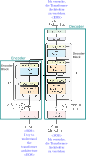
\includegraphics[width=.5\textwidth]{figures/transformer_architecture}
	\caption{Die Modell-Architektur des Transformers (siehe \cite{Attention_is_all_you_need}, leicht modifiziert).}
	\label{Abb:transformer_architecture}
\end{figure}
Um alle Teilschichten herum werden sogenannte \emph{Residualverbindungen}\footnote{Die Verwendung von Residualverbindungen im Transformer dient primär dazu, zwei wesentliche Herausforderungen in tiefen neuronalen Netzen zu bewältigen. Erstens ermöglichen die Residualverbindungen einen reibungslosen Gradientenfluss während des Trainings, indem sie das Problem des Verschwindens oder Explodierens von Gradienten mindern. Dadurch wird das Training komplexer Modelle effizienter und stabiler. \footcite{Residual_Connections} Zweitens bewahren die Residualverbindungen die Informationen über die ursprüngliche Sequenz, welche ansonsten durch die Multi-Head-Aufmerksamkeitsschicht teilweise verloren gehen könnten (wird später erläutert werden) \footcite{Attention_is_all_you_need}\todo{Schauen, ob das wirklich erläutert wird}. Dies gewährleistet, dass die Ausgabevektoren der einzelnen Positionen der Sequenz relevante Beziehungen zu ihren Eingabeelementen beibehalten. Somit tragen die Residualverbindungen dazu bei, sowohl den Gradientenfluss als auch die Kontextualisierung der Eingabeinformationen im Transformer zu optimieren und eine präzise Modellierung komplexer Abhängigkeiten zu ermöglichen.} verwendet, gefolgt von einer Schichtnormalisierung (\emph{engl. „layer normalization“}). Das bedeutet, dass die Ausgabe jeder Teilschicht $$LayerNorm(x + Sublayer(x))$$ ist, wenn $x$ die Eingabedaten derselben Teilschicht darstellt. Um diese Residualverbindungen zu ermöglichen, erzeugen alle Teilschichten im Modell sowie die Einbettungsschichten (hierauf wird im Folgenden noch eingegangen werden) Ausgaben mit der Dimension $d_{model}=512$.

Im Folgenden werden die grundlegenden Bausteine neuronaler Netze (Funktionen mit erlernbaren Parametern; vgl. \cite{Formal_Algorithms_for_Transformers_DeepMind}) - beginnend mit der Verarbeitung der Eingabesequenz „I try to understand the Transformer architecture“ - vorgestellt, aus denen die Transformer aufgebaut sind. Ziel ist es, die Funktionsweise der Transformer schrittweise zu erläutern, indem die Betrachtung von der abstrakten Gesamtarchitektur abweicht und stattdessen die einzelnen Komponenten bzw. Bausteine, wie sie in \cref{Abb:transformer_architecture} dargestellt sind, im Detail betrachtet werden. Zuerst sollen demnach die internen Komponenten des Encoders genauer untersucht werden. 
\todo{Wie soll es aufgebaut werden? In Originalpaper sind Input und Output in einem erklärt und genauso in DeepMind-Paper. Auch so machen und Überschrift „Embedding“ verwenden oder getrennt?}

\subsection*{Encoder}
Wie in der \cref{Abb:transformer_architecture} links unten zu sehen, besteht der erste Schritt in der Umwandlung der Eingabedaten in sogenannte \emph{Input-Embeddings} (Eingabe-Einbettungen). 

\subsubsection*{Input-Embedding}

Im Allgemeinen dienen die Embeddings dazu, jedes Element des \emph{Vokabulars} als Vektoren der Dimension $d_{model}$ darzustellen. Im Kontext des Übersetzungsbeispiels bezieht sich das Vokabular auf die Menge aller Wörter, Buchstaben oder Teilwörter, die auch als \emph{Tokens} bezeichnet werden, und die in der Sprache oder im Textkorpus vorhanden sind, mit dem der Transformer trainiert wird. Üblicherweise werden Teilwörter als Tokens verwendet, aber für diese Arbeit sollen aus Gründen der Einfachheit vollständige Wörter als Tokens dienen. Somit umfasst das Vokabular im Beispiel alle englischen und deutschen Wörter und jedes Element dieses Vokabulars erhält einen eindeutigen Index. Hinzu kommen noch ein paar Spezialtoken wie das <SOS>-Token („\emph{Start Of Sentence}“) und das <EOS>-Token („\emph{End Of Sentence}“) zur Kennzeichnung des Starts bzw. Endes einer Sequenz, sowie ein Masking-Token, das später im Decoder benötigt wird. \cite{Formal_Algorithms_for_Transformers_DeepMind}

Die Eingabesequenz „I try to understand the Transformer architecture“ würde nach einer Tokenisierung (\emph{engl. „Tokenization“}) auf Wortebene daher (bei Vernachlässigung der Spezialtokens) die folgenden sieben Elemente beinhalten:
$$[\text{'I', 'try', 'to', 'understand', 'the', 'Transformer', 'architecture'}].$$

Da Computer nicht direkt mit Worten arbeiten können, erfolgt im nächsten Schritt die Umwandlung der Eingabesequenz in eine Sequenz von Zahlen. Diese Zahlen entsprechen den Indizes der entsprechenden Wörter im Vokabular und werden als \emph{„Token-IDs“} bezeichnet sowie innerhalb der Sequenz zwischen die IDs des <SOS>- und <EOS>-Tokens eingebettet\footnote{Achtung! Die Wahl und Verwendung/Platzierung der Spezialtokens wird in der Literatur sowie in praktischen Implementierungen des Transformers unterschiedlich gehandhabt und ist zudem abhängig von der jeweiligen Aufgabenstellung (siehe z.B. \cite{Transformer_Implementation_Google_Tensor2Tensor}, \cite{Transformer_Implementation_Harvard} oder \cite{Transformers_HuggingFace_Natural_Language}). Insbesondere bei Übersetzungsaufgaben bedient sich der Transformer häufig der Spezialtokens <SOS> und <EOS>. Diese dienen dazu, den Anfang und das Ende einer Übersetzung festzulegen und dem Modell somit zu signalisieren, wann es mit der Übersetzung beginnen bzw. sie abschließen soll. Die Verwendung solcher Tokens trägt dazu bei, dass das Modell den Kontext und die Abgrenzung der Übersetzung besser erfasst und erlernt. Die in diesem Bericht verwendeten Erläuterungen und Visualisierungen orientieren sich an einer leicht verständlichen \emph{From-Scratch-}Implementierung, die auf GitHub zur Verfügung steht (siehe \href{https://github.com/hkproj/pytorch-transformer}{https://github.com/hkproj/pytorch-transformer}) und auf der Transformer-Architektur, wie sie im „\emph{Attention Is All You Need}“-Paper vorgestellt wurde, basiert. Demnach ist - wie aus \cref{Abb:transformer_architecture} hervorgeht - die Input-Sequenz des Encoders zwischen diese beiden speziellen Tokens eingebettet. Der Input-Sequenz des Decoders wird lediglich das <SOS>-Token vorangestellt, und dem Output das <EOS>-Token hinzugefügt.} \cite{Formal_Algorithms_for_Transformers_DeepMind}. 

Zu diesem Zeitpunkt können die Eingabewörter zwar durch die Token-IDs identifiziert werden, jedoch besitzen die IDs ansonsten keine semantische Bedeutung. Um den Wörtern eine Bedeutung zuzuordnen, wird eine sogenannte \emph{„Embedding-Matrix“} verwendet.  Hierfür werden die Token-IDs aller Elemente des Vokabulars in Vektoren der Größe $d_{model}$ umgewandelt und diese Vektoren bilden schließlich die Embedding-Matrix mit der Dimension $(N_V, d_{model})$, wobei $N_V$ die Anzahl der Elemente im Vokabular angibt. Der Transformer erhält dann als Input eine Matrix der Größe $(n, d_{model})$, die die zu den Eingabewörtern gehörigen Embeddings enthält, und $n$ bezeichnet weiterhin die Länge der Eingabesequenz\todo{Achtung! Schauen, ob das so stimmt und n nach wie vor die Anzahl der Eingabeelemente darstellt ($x_1, ..., x_n$)}. Tritt dasselbe Wort mehrfach in der Eingabesequenz auf, so ist der entsprechende Embedding-Vektor jedes Mal identisch. Während die Token-IDs feststehen und sich nicht ändern, sind die Embedding-Vektoren variabel, da ihre Werte Modellparameter sind. Im Verlauf des Trainings werden sich diese Werte entsprechend der Verlustfunktion (\emph{engl. „loss function“}) ändern, um gewissermaßen die Bedeutung der einzelnen Worte adäquat zu repräsentieren. Der lila eingefärbte Kasten in \cref{Abb:TransformerVisualization} verdeutlicht den Prozess des Input-Embeddings\todo{Achtung! Schauen ob der Satz dann noch zu Grafik passt, oder ob Grafik nicht deutlich mehr abdeckt}. Aus Gründen der Übersichtlichkeit wurde hier bewusst auf die Visualisierung der Special-Tokens verzichtet\footnote{In der Praxis haben die Input- und Outputsequenzen des Transformers eine einheitliche, vorab festgelegte Länge (typischerweise die Länge des längsten Satzes innerhalb der Trainingsmenge inkl. der Spezialtokens). Das liegt daran, dass die Größe der Gewichtsmatrizen im Transformer für unterschiedliche Sätze nicht einfach vergrößert oder verkleinert werden kann. Ist ein Satz zu kurz, so wird er mit sogenannten „\emph{padding}“-Tokens aufgefüllt, bis er die erwartete, festgelegte Länge erreicht. Für mehr Informationen siehe \emph{„transformer\_embedding.ipynb“}.} sowie auf die Verwendung konkreter Zahlenwerte. Daher wird dieser Arbeit ergänzend ein Jupyter Notebook namens \emph{„transformer\_embedding.ipynb“} beigelegt, das auf der Transformers-Bibliothek von HuggingFace \cite{Transformers_HuggingFace_Natural_Language} beruht und sowohl das Input-Embedding zeigt, als auch den umgekehrten Prozess nach Anwendung des Transformers, wenn die Embeddings wieder in ein für den Menschen lesbares Format gebracht werden (das in diesem Fall die Übersetzung enthält). 

\todo{Padding erklären und dass verwendet bei Batches, in denen Sätze mit unterschiedlicher Länge stehen (vermutlich nicht visualisieren oder nur ausbleichen $\rightarrow$ hängt mit der $seq\_len$ zusammen. Diese ist dann normalerweise festgelegt und der Rest wird mit padding aufgefüllt. Siehe Teams)}


\subsubsection*{Positional Encoding}

Das Transformer-Modell zeichnet sich - wie bereits erwähnt - durch das Fehlen sowohl von rekurrenten Netzen als auch von Faltungsnetzen aus. Daher ist es erforderlich, Informationen über die relative oder absolute Position der Tokens in der Sequenz hinzuzufügen, um die Reihenfolge der Elemente in der Sequenz sinnvoll nutzen zu können. Ein markantes Merkmal des Transformers besteht darin, dass bei Vertauschung zweier Eingabeelemente, wie beispielsweise den Tokens „I“ und „try“, das Ergebnis im Wesentlichen gleich bleibt, abgesehen von den beiden vertauschten Elementen. Diese Eigenschaft, die als Permutationsinvarianz bezeichnet wird, stellt einen der größten Vorteile des Transformer-Modells dar, da sie die parallele Verarbeitung des gesamten Eingabetextes ermöglicht. Jedoch geht hierdurch die Information über die ursprüngliche Anordnung der Wörter im Satz verloren. Dies wird deutlicher anhand eines Beispiels: Die Sätze „I am learning how transformers work“ und „Am I learning how transformers work“ beinhalten exakt dieselben Wörter, haben aber eine andere Bedeutung. Der erste Satz ist eine Aussage. Der zweite jedoch eine Frage. Dies verdeutlicht die Herausforderung, die Positionsinformationen in das Modell zu integrieren, um eine sinnvolle Verarbeitung von Sequenzen zu gewährleisten.

Die Autoren von \cite{Attention_is_all_you_need} lösen dieses Problem, indem sie zu den Input Embeddings sogenannte \emph{„Positional Encodings“} (Positionskodierungen) addieren. Folglich haben die Positionskodierungsvektoren dieselbe Dimension $d_{model}$ wie die Embeddings. \cref{Abb:TransformerVisualization} zeigt dieses Vorgehen. So ist zu erkennen, dass sich der in grau dargestellte Input für den ersten Encoder-Block aus dem Input-Embedding (lila) sowie dem Positional Encoding (blau) zusammensetzt. Diese Vektoren werden einmal berechnet und nicht während des Trainingsprozesses erlernt\footnote{In der Literatur gibt es unterschiedliche Möglichkeiten, Positional Encodings durchzuführen \cite{Formal_Algorithms_for_Transformers_DeepMind}\cite{Goodfellow_Handbuch}\cite{PositionalEncodingTransformers}. Neben den festen Embeddings, wie sie von \cite{Attention_is_all_you_need} verwendet werden, gibt es auch Embeddings, die während der Trainingsphase vom Modell erlernt werden \cite{Conv_Seq2Seq_Learning}. Im „Attention Is All You Need“-Paper zeigen die Verfasser auf, dass beide Herangehensweisen vergleichbare Resultate erzielen. Sie präferierten jedoch die festen Positionskodierungen, da sie mutmaßten, dass diese dem Modell möglicherweise erlauben, auch auf Sequenzlängen zu generalisieren, die über die im Training bekannten hinausgehen.}. Jeder der $512$-dimensionalen Vektoren repräsentiert die Position des jeweiligen Wortes bzw. Tokens innerhalb des Satzes und zur Berechnung der Positional Encodings verwenden die Autoren Sinus- und Cosinus-Funktionen\footnote{Auf den ersten Blick könnte man in Betracht ziehen, einen einfachen indexbasierten Ansatz zu verwenden, um die Positionen von Elementen in einer Sequenz darzustellen. Zum Beispiel könnten aufeinanderfolgende Ganzzahlen wie $0, 1, 2, 3, ...$ (bzw. $512$-dimensionale Vektoren, die jeweils nur aus einer dieser ganzen Zahlen aufgespannt werden) verwendet werden, um die Positionen von Wörtern in einem Satz darzustellen. Das führt jedoch zu Problemen, denn wenn linear steigende Positionswerte zu den Input Embeddings hinzugefügt werden, erhalten Wörter am Satzanfang kleine Werte, während Wörter am Satzende große Werte haben. Dies kann zu einem Bias (\emph{dt. „Verzerrung“}) im Modell führen, da Wörter am Satzende übermäßig stark gewichtet werden. Darüber hinaus würde die Verwendung solcher kontinuierlichen Zahlen dafür sorgen, dass das Modell bei einer Eingabesequenz aus mehreren Sätzen annimmt, dass die Sätze immer gleichzeitig auftreten. Die Normalisierung der Positionswerte, um Werte zwischen $0$ und $1$ zu erhalten, könnte eine Lösung für das Problem sein. Doch da diese Zahlen je nach Länge des Satzes erzeugt werden, würden die Zahlenwerte mit einer Änderung der Satzlänge variieren und damit würde man derselben Position eine unterschiedliche Zahl zuordnen.} unterschiedlicher Frequenzen: 

\begin{equation}\label{eq:PosEncode}
	\begin{aligned}
		PE_{pos,2i} &= \sin\left(\frac{pos}{10000^{\frac{2i}{d_{model}}}}\right)\\
		PE_{pos,2i+1} &= \cos\left(\frac{pos}{10000^{\frac{2i}{d_{model}}}}\right)
	\end{aligned}
\end{equation}

Dabei bezeichnet \emph{pos} die Position des Wortes bzw. Tokens in der Eingabesequenz und \emph{i} die Dimension innerhalb des $d_{model}$-dimensionalen Encoding-Vektors. Durch die Verwendung dieser trigonometrischen Funktionen kann das Modell lernen, wie Wörter in verschiedenen Abständen zueinander liegen. Terme in den unteren Dimensionen - also den ersten Stellen in den Vektoren - haben kurze Wellenlängen, die in den höheren Dimensionen längere. Die unterschiedlichen Frequenzen ermöglichen es dem Modell, Informationen über die relative Positionierung der Wörter zu extrahieren. Dies trägt dazu bei, dass das Modell Wörter, die nah beieinander stehen, als nahe und Wörter, die entfernt voneinander sind, als distanziert erkennt und dass jede Position in der Sequenz (im Beispiel jedes Wort) eine einzigartige Kombination von Sinus- und Cosinus-Termen erhält, die ein charakteristisches Muster erzeugt. Dadurch kann das Modell flexibel auf unterschiedliche (noch nicht im Training gesehene) Eingabegrößen und -längen reagieren und dennoch die semantische Bedeutung von Texten erfassen. 

Die blau eingefärbte Gedankenwolke\footnote{Siehe beigelegtes Notebook namens \emph{„transformers\_positional\_encoding.ipynb“} zum Experimentieren mit den Positional Encodings.} in \cref{Abb:TransformerVisualization} soll veranschaulichen, wie die Encoding Vektoren zustande kommen. Dargestellt sind die ersten vier der insgesamt $d_{model}=512$ Sinus-/Cosinusschwingungen. Jede dieser Schwingungen liefert spezifische Positionswerte für das Embedding jedes Wortes/Tokens in der Eingabesequenz. Die x-Achse repräsentiert dabei die Wortpositionen, die sieben Werte für die sieben Eingabetokens umfassen. Die y-Achsen liefern die Werte der Positional Encodings für jede Dimension $i$. Als Beispiel liefern die y-Werte der ersten (blauen) Schwingung die Positionskodierungswerte für die ersten Einbettungen jedes Wortes, wodurch die erste Spalte der Positionskodierungsmatrix gefüllt wird. Entsprechend setzt sich die erste Zeile der Matrix, die der Kodierung des Wortes „I“ entspricht, aus allen $512$ y-Werten zusammen, die sich an der Position $pos=0$ befinden, wie schemenhaft durch die farbigen Punkte zu Beginn des ersten Positionskodierungsvektors in der Abbildung dargestellt. Des Weiteren verdeutlicht die Visualisierung, dass die Wellenlängen mit zunehmender Dimension ansteigen (die grüne und rote Schwingung, die den Dimensionen $i=2$ und $i=3$ entsprechen, haben längere Wellenlängen als die blaue und orangene Schwingung, die die Kodierungen niedrigerer Dimensionen zeigen).

\begin{figure}
	\centering
	\includesvg[width=\textwidth]{figures/TransformerVisualization}
	\caption{Veranschaulichung der ersten beiden Transformer-Bausteine anhand des Beispielsatzes „I try to understand the Transformer architecture“. Im Verlauf der Input-Embedding-Phase (in lila hervorgehoben) werden den einzelnen Wörtern bzw. Tokens im Satz sogenannte Token-IDs zugewiesen und daraufhin $d_{model}=512$-dimensionale Repräsentationen, auch als Embeddings bezeichnet, erzeugt. Diese Embedding-Vektoren repräsentieren die semantische Bedeutung der Eingabewörter. Zusätzlich zu den Input-Embeddings werden sogenannte Positional Encodings generiert (siehe blauer Kasten), welche die Information über die Position eines Wortes im Eingabesatz enthalten. Die blau eingefärbte Gedankenwolke veranschaulicht, wie die einzelnen Werte der Positionskodierungsvektoren ermittelt werden. Die resultierende, grau gekennzeichnete Matrix stellt den Input für den ersten Encoder-Block dar.}
	\label{Abb:TransformerVisualization}
\end{figure}


\subsubsection*{Multi-Head-Attention}

Der Aufmerksamkeits-Mechanismus ist die zentrale architektonische Komponente von Transformern. Dieser befähigt neuronale Netzwerke, kontextbezogene Informationen wie vorangehenden oder umgebenden Text zu nutzen, um das aktuelle Token vorherzusagen. \cite{Formal_Algorithms_for_Transformers_DeepMind} Im \emph{„Attention Is All You Need“}-Paper wird ein spezifischer Aufmerksamkeitsmechanismus namens \emph{„Selbstaufmerksamkeit“} verwendet. Dieser Mechanismus erlaubt es dem Modell, Beziehungen zwischen den Wörtern eines Textes zu etablieren. Um ein tiefergehendes Verständnis zu ermöglichen, wird zunächst die \emph{Single-Head-Attention} erläutert, bevor die \emph{Multi-Head-Attention} behandelt wird.

Das grundlegende Konzept umfasst die sogenannten \emph{Abfragen (Queries)}, \emph{Schlüssel (Keys)} und \emph{Werte (Values)}, die alle in Form von Vektoren vorliegen. Dazu werden zunächst drei Kopien des Encoder Inputs gemacht - sprich die einzelnen Vektoren entsprechen lediglich den Tokendarstellungen des Eingabesatzes, die sich nach dem Input-Embedding und Positional Encoding ergeben haben\footnote{In \cref{Abb:TransformerVisualization} wurde bereits die Funktionsweise der ersten beiden Transformerbausteine visualisiert. Der erste (grau dargestellte) Vektor im Encoder Input entspricht hier einer $d_{model}=512$-dimensionalen Repräsentation des Tokens „I“ aus dem Eingabesatz, nachdem sowohl das Input Embedding als auch das Positional Encoding darauf angewendet wurden. Dementsprechend sind der erste Query-, Key- und Value-Vektor jeweils Kopien dieses ersten Encoder Inputs.} \cite{Mathematical_view_of_attention_models_in_deep_learning}. Dann wird das Skalarprodukt zwischen der Abfrage und allen Schlüsselvektoren (einschließlich des Schlüssels desselben Wortes) gebildet, um die Kompatibilität - einen sog. \emph{Score} - zwischen z.B. dem Wort „I“ und den übrigen Wörtern des Eingabesatzes zu bestimmen. Dieser Score quantifiziert den Grad, in dem ein Wort seinen Fokus auf andere Wörter im Satz legen sollte bzw. beschreibt, wie wichtig ein Token für die Vorhersage eines anderen Tokens ist. Ein höherer Scorewert impliziert dabei eine intensivere Beachtung\footnote{Um die Bedeutung dieses Schritts hervorzuheben und das Verständnis des Lesers zu stärken, sollen die Sätze „The animal didn't cross the street because it was too tired.“ und „The animal didn't cross the street because it was too wide.“ aus dem Blog-Post \url{https://blog.research.google/2017/08/transformer-novel-neural-network.html} von Google Research herangezogen werden. Hier wird illustriert, wie der Transformer eine herausfordernde Aufgabe der maschinellen Übersetzung bewältigt, nämlich die Unterscheidung, dass sich im ersten Satz das Wort „it“ auf das Tier und im zweiten auf die Straße bezieht. Diese Unterscheidung ist wesentlich, da bei der Übersetzung in z.B. die deutsche Sprache die Wörter „Tier“ und „Straße“ unterschiedliche Geschlechter aufweisen, wodurch die Übersetzung von „it“ vom Geschlecht des Substantivs abhängt. Eine sinnbildliche Darstellung der Wörter, auf die der Encoder während der Berechnung der endgültigen Darstellung für das Wort „it“ achtet, ist in dem besagten Blog-Post zu finden. Der Transformer erkennt eindeutig die beiden Substantive, auf die sich „it“ beziehen könnte, und die jeweilige Hervorhebung der Aufmerksamkeit in verschiedenen Blautönen spiegelt seine Wahl in den unterschiedlichen Kontexten wider. Die besagte Visualisierung kann ebenfalls \cref{Abb:attention_google} entnommen werden. Zusätzlich bietet \url{https://colab.research.google.com/github/tensorflow/tensor2tensor/blob/master/tensor2tensor/notebooks/hello_t2t.ipynb} die Möglichkeit, ein Transformermodell zu laden und anschließend ein besseres Verständnis für den Aufmerksamkeitsmechanismus zu erlangen mithilfe von interaktiven Visualisierungen. Dort ist ebenfalls das genannte Beispiel zu finden, allerdings kann man zusätzlich sehen, auf welche Worte andere Aufmerksamkeitsköpfe des Transformers ihre Aufmerksamkeit richten.}. 

In der Praxis wird die Aufmerksamkeitsfunktion simultan für alle Abfragen (und somit für die Repräsentationen aller Wörter) berechnet, wie in \cref{Abb:Selfattention} dargestellt. Dabei erfolgt die Verarbeitung nicht mit individuellen Vektoren, die die Repräsentation eines einzelnen Wortes beschreiben, sondern mittels der Matrizen $Q,\ K$ und $V$. Diese Matrizen repräsentieren den gesamten Eingabesatz, der in der Abbildung durch die $n$ grauen, $d_{model}$-dimensionalen Vektoren gegeben ist, die die Einbettungs- und Positionskodierungsinformationen enthalten (vgl. \cref{Abb:TransformerVisualization}). Somit ergibt sich die Score-Matrix aus der Matrixmultiplikation $QK^T$. Hier wird auch der Grund für die Bezeichnung dieser Form der Aufmerksamkeit als \emph{Selbstaufmerksamkeit}\footnote{Die beschriebene Selbstaufmerksamkeit ist nicht der einzig mögliche Aufmerksamkeitsmechanismus. Es gibt beispielsweise auch die Aufmerksamkeit mit einer erlernbaren Query. Diese Variante unterscheidet sich hauptsächlich in der Art und Weise, wie die Matrizen $Q,\ K$ und $V$ erhalten werden. In der Selbstaufmerksamkeit wird die Intra-Korrelation einer gegebenen Eingabematrix $X$ erfasst, wobei $Q=K=V=X$ gilt. Bei der Aufmerksamkeit mit erlernbarer Abfrage hingegen bleibt $K=V=X$, jedoch wird die Abfrage $Q$ weder als Eingabe gegeben, noch ist sie von der Eingabe abhängig. Stattdessen werden die Einträge der Matrix $Q$ direkt als trainierbare Variablen gelernt. \footcite{Mathematical_view_of_attention_models_in_deep_learning}} erkenntlich: Die resultierende Matrix beschreibt, wie jedes Wort des Eingabesatzes mit jedem anderen in Beziehung steht. So beschreibt das Element in Zeile 1 und Spalte 1 der Score-Matrix gewissermaßen, wie sehr das Wort „I“ auf sich selbst achtet. Das Matrixelement in Zeile 2 und Spalte 4 enthält analog das Skalarprodukt von der Repräsentation des Wortes „try“ mit der Repräsentation des Wortes „understand“. Um die Gradienten zu stabilisieren und mögliche explosionsartige Effekte zu verhindern\footnote{Die Autoren in \footcite{Attention_is_all_you_need} vermuteten, dass bei einer großen Dimensionalität $d_k$ der Abfrage- und Schlüsselvektoren die Skalarprodukte in ihrer Größenordnung zunehmen, was die Softmax-Funktion in Bereiche mit extrem kleinen Gradienten verschiebt.}, werden die Scores durch die Quadratwurzel der Dimensionalität $d_k$ der Abfragen und Schlüssel (diese Dimensionalität entspricht im Falle der \emph{Single-Head-Attention} der Modelldimension $d_{model}=512$) geteilt. Anschließend wird die Softmax-Funktion angewendet, um skalierte Scores zu erhalten, die als Aufmerksamkeitsgewichte in Form von Wahrscheinlichkeitswerten zwischen null und eins vorliegen. Die Zeilen der erzeugten Score-Matrix summieren jeweils zu eins. Schließlich werden die Aufmerksamkeitsgewichte verwendet, um die Wertmatrix zu gewichten. Dadurch werden relevante Informationen betont, während der Einfluss irrelevanter Wörter reduziert wird. Auf dieser Weise gewährleistet das Modell präzise Vorhersagen basierend auf dem Kontext. Die Zeilen der resultierenden Ausgabematrix beschreiben folglich nicht mehr nur die Bedeutung oder Position eines Wortes im Eingabesatz, sondern auch die Beziehung eines Wortes zu den anderen. So könnte die neue Darstellung des Wortes „Transformer“ aus dem Eingabesatz beispielsweise widerspiegeln, dass es sich um die Architektur eines neuronalen Netzes und nicht um einen Science-Fiction-Spielfilm handelt. Die Formel zur Berechnung der Selbstaufmerksamkeit lautet \begin{equation}\label{eq:SelfAttention}
	Attention(Q,K,V)=softmax(\frac{QK^T}{\sqrt{d_k}})V
\end{equation}

\begin{figure}
	\centering
	\includesvg[width=\textwidth]{figures/Selfattention}
	\caption{Graphische Darstellung der Selbstaufmerksamkeit im ersten Encoder-Block. Dabei symbolisiert das Zeichen $\times$ die Matrixmultiplikation und $softmax()$ repräsentiert den Softmax-Operator, der auf die Zeilen angewendet wird. Die Matrizen $Q,K$ und $V$ entsprechen Kopien der Eingangsmatrix, die nach Anwendung des Input-Embeddings und Positional-Encodings entsteht. Für jede Zeile in $Q$ und jede Spalte in $K^T$ wird ein Ähnlichkeitswert (Score) berechnet. Durch die Anwendung der Softmaxfunktion werden diese Werte normalisiert und addieren sich zu 1. Das Matrixprodukt der normalisierten Werte mit der Matrix $V$ ergibt die entsprechende Ausgabematrix.}
	\label{Abb:Selfattention}
\end{figure}

Anstatt eine einzelne Aufmerksamkeitsfunktion mit $d_{model}$-dimensionalen Queries, Keys und Values zu berechnen, stellten die Autoren von \cite{Attention_is_all_you_need} fest, dass es von Vorteil ist, die Abfragen, Schlüssel und Werte nicht einmal, sondern $h$ Mal mit unterschiedlichen, erlernten linearen Projektionen auf $d_k,\ d_k$ und $d_v$ Dimensionen zu projizieren\footnote{Im Originalpaper \cite{Attention_is_all_you_need} werden $h=8$ parallel arbeitende Aufmerksamkeitsschichten bzw. -Köpfe verwendet, sodass $d_k=d_v=\frac{d_{model}}{h}=64$. Aufgrund der reduzierten Dimension jedes Kopfes ist der Gesamtberechnungsaufwand ähnlich wie bei der Aufmerksamkeitsberechnung mit nur einem einzigen Kopf bei voller Dimensionalität.} (die Abfrage- und Schlüsselvektoren haben wegen des Skalarprodukts dieselbe Dimension). Diese \emph{Multi-Head-Attention} ermöglicht es dem Modell durch die Verwendung mehrerer Aufmerksamkeitsköpfe verschiedene Darstellungen gleichzeitig zu lernen. Auf jeder dieser projizierten Versionen von Queries, Keys und Values wird die Aufmerksamkeitsfunktion \ref{eq:SelfAttention} dann parallel ausgeführt, was $d_v$-dimensionale Ausgabewerte ergibt. Anschließend werden die Ausgabewerte wieder aneinander konkateniert und erneut projiziert, was zu den endgültigen Aufmerksamkeitswerten führt. In Formeln ausgedrückt bedeutet dies:

\begin{equation}\label{eq:multiheadattention}
	\begin{aligned}
		MultiHead(Q,K,V) &= Concat(head_1, ..., head_h)W^O\\
		\text{wobei } head_i &= Attention(QW_i^Q, KW_i^K, VW_i^V)
	\end{aligned}
\end{equation}

Die Projektionen sind hier die Parameter- /Gewichtsmatrizen $W_i^Q\in \mathbb{R}^{d_{model}\times d_k}, W_i^K\in \mathbb{R}^{d_{model}\times d_k}, W_i^V\in \mathbb{R}^{d_{model}\times d_v}$ sowie $W^O\in \mathbb{R}^{h d_v\times d_{model}}$.

Das beschriebene Vorgehen ist in \cref{Abb:MultiheadAttention} veranschaulicht sowie im dieser Arbeit beigelegten Notebook namens \emph{„transformers\_attention.ipynb“} Schritt für Schritt detailliert demonstriert. Kurz gesagt projiziert die Multi-Head-Attention die Abfragen, Schlüssel und Werte mehrfach in verschiedene Unterräume und führt in jedem dieser Unterräume separat die Aufmerksamkeitsfunktion aus, wie anhand der Abbildung deutlich wird. Dieser erweiterte Aufmerksamkeitsmechanismus ermöglicht es dem Modell, unterschiedliche Arten von Informationen oder Beziehungen in den Eingabedaten zu erkennen und zu verarbeiten, indem es unterschiedliche Aspekte der Daten in verschiedenen Repräsentationsunterräumen gleichzeitig berücksichtigt und in die endgültige Repräsentation mit einfließen lässt. Dies liegt daran, dass jeder Kopf auf seinen eigenen projizierten Vektoren operiert, wodurch das Modell unterschiedliche Perspektiven oder „Sichten“ auf dieselben Eingabedaten erhält. Das ist insbesondere nützlich, um komplizierte Abhängigkeiten wie die Kontextabhängigkeit von Pronomen in natürlichen Sprachen zu modellieren, was die Effektivität des Transformer-Modells in Aufgaben wie maschineller Übersetzung und Textgenerierung maßgeblich erhöht \cite{BERT}\cite{WNLI}. Im Vergleich zur Single-Head-Attention, die gewisse Aspekte des Inputs über- oder unterbewerten könnte, bietet die Multi-Head-Attention eine umfassendere und nuanciertere Betrachtungsweise.

\begin{landscape}
\begin{figure}
	\centering
	\includesvg[width=\linewidth]{figures/MultiheadAttention}
	\caption{Schematische Darstellung des Multi-Head-Attention-Mechanismus innerhalb eines Transformers. Zuerst wird gezeigt, wie die einzelnen Wörter (Zeilen) des Encoder-Inputs in Vektoren für Anfragen, Schlüssel und Werte kopiert werden, die die Basis für die Matrizen $Q$, $K$ und $V$ bilden. Durch die Verwendung der Gewichtsmatrizen $W^Q$, $W^K$ und $W^V$ gehen die Input-Repräsentationen in die entsprechenden Projektionen $Q^\prime$, $K^\prime$ und $V^\prime$ über. Diese projizierten Tensoren dritter Stufe repräsentieren die Aufteilung der Eingabeinformationen auf verschiedene Aufmerksamkeitsköpfe. Jeder Aufmerksamkeitskopf verarbeitet diese Projektionen separat durch Anwendung der Aufmerksamkeitsfunktion \ref{eq:SelfAttention}, woraufhin die resultierenden Vektoren jedes Kopfes jeweils zu einem einzigen Vektor konkateniert und durch eine weitere Gewichtsmatrix $W^O$ in den endgültigen Aufmerksamkeits-Output transformiert werden. Erläuterungen zu den verwendeten Operationen und Notationen sind den grau hinterlegten Bereichen der Visualisierung zu entnehmen.}
	\label{Abb:MultiheadAttention}
\end{figure}
\end{landscape}



\subsubsection*{Feed-Forward}

Im Kontext der Transformer-Architektur ermöglichen die positions-weisen \textbf{F}eed-\textbf{F}orward-\textbf{N}etze (\emph{FFN}) eine zusätzliche Abstraktionsebene über die durch die Aufmerksamkeitsmechanismen gewonnenen Informationen. So spielt z.B. die Feed-Forward Schicht innerhalb des Encoders eine essentielle Rolle für die weitere Aufbereitung der durch den Selbstaufmerksamkeitsmechanismus vorverarbeiteten Eingabesequenz. Sie setzt sich aus zwei aufeinanderfolgenden linearen Transformationen mit einer dazwischengeschalteten nicht-linearen ReLU-Aktivierungsfunktion (\emph{\textbf{Re}ctified \textbf{L}inear \textbf{U}nit}) zusammen. Diese Schicht appliziert für jede Position der Eingabesequenz eine unabhängige und identische vollständig verbundene Schicht. Jedes Wort bzw. jedes Token in der Sequenz wird durch diese Transformation individuell verarbeitet, was eine differenzierte Repräsentation der Tokens ermöglicht. Formal ausgedrückt wird die Operation eines FFN durch die Gleichung
\begin{equation}\label{eq:FFN}
	FFN(x) = max(0, xW_1 + b_1)W_2+b_2
\end{equation}
dargestellt, wobei $W_1$ und $W_2$ Gewichtsmatrizen und $b_1$ und $b_2$ Bias-Vektoren sind. Zwar sind die linearen Transformationen für unterschiedliche Positionen der Sequenz identisch, allerdings nutzen sie von Schicht zu Schicht unterschiedliche Parameter. Die erste Transformation projiziert die Eingabedaten in einen höherdimensionalen Raum mit der Dimensionalität $d_{ff}=2048$ (vgl. \cite{Attention_is_all_you_need}), was dem Modell ermöglicht, komplexere Muster zu erfassen. Die ReLu-Aktivierung fügt Nichtlinearität hinzu, was entscheidend ist, um komplexe Abhängigkeiten innerhalb der Daten zu modellieren. Die zweite Transformation komprimiert die durch die ReLU-Funktion aktivierten Daten zurück in den Raum der ursprünglichen Dimension $d_{model}=512$.\footnote{Für den interessierten Leser sei auf \footcite{TransformerFeedForward} verwiesen. Dort untersuchen Mor Geva, Roei Schuster, Jonathan Berant und Omer Levy die Rolle der Feed-Forward-Schichten in Transformer-basierten Sprachmodellen. Die Autoren argumentieren, dass diese Schichten als eine Art Key-Value-Speicher operieren, wobei jeder „Key“ mit textuellen Mustern in Trainingsbeispielen korreliert und jeder „Value“ eine Verteilung über das Ausgabevokabular induziert. Die Studie zeigt, dass die in den Feed-Forward-Schichten gelernten Muster für Menschen interpretierbar sind und dass untere Schichten eher oberflächliche Muster erfassen, während obere Schichten tiefere semantische Muster lernen. Abschließend stellen die Autoren fest, dass die Ausgabe einer Feed-Forward-Schicht eine Zusammensetzung seiner Erinnerungen ist, die durch residuale Verbindungen im Modell verfeinert wird, um die endgültige Ausgabe-Verteilung zu erzeugen.}

Nachdem die Input-Embeddings, Positional Encodings, Multi-Head-Attention und Feed-Forward-Schichten durchlaufen wurden, ist der Prozess einer Encoder-Schicht abgeschlossen. Dieser gesamte Vorgang wird im Transformer-Modell jedoch nicht nur einmal, sondern insgesamt sechs Mal (vgl. \cref{Abb:transformer_architecture}) wiederholt. Jede Wiederholung besteht aus einer weiteren Encoder-Schicht, die auf den Ausgaben der vorherigen Schicht aufbaut und die Eingabedaten schrittweise weiter verarbeitet und verfeinert. Durch diese iterative Verarbeitung kann das Modell zunehmend tiefere und komplexere Beziehungen innerhalb der Eingabedaten erkennen und abbilden. Der Output der letzten Encoder-Schicht, ein hochgradig kontextualisiertes und abstrahiertes Abbild der ursprünglichen Eingabesequenz, wird dann an den Decoder-Teil des Transformers weitergeleitet. Im Decoder erfolgt eine ähnliche, jedoch leicht modifizierte Verarbeitung, die zusätzlich von den Informationen aus dem Encoder beeinflusst wird, um letztendlich die Zielübersetzung oder Ausgabe zu generieren. Im Folgenden sollen daher bei der Erklärung der Decoder-Komponenten hauptsächlich die Unterschiede zu denen des Encoders hervorgehoben werden. Da das Positional Encoding sowie die Feed-Forward-Schicht des Decoders komplett identisch zu den entsprechenden Schichten des Encoders erfolgen, wird hierauf nicht noch einmal eingegangen.

\subsection*{Decoder}
Wie aus \cref{Abb:transformer_architecture} hervorgeht, startet der Decoder mit dem sog. \emph{Output-Embedding}.

\subsubsection*{Output-Embedding}

Das Output-Embedding im Decoder des Transformers unterscheidet sich in einem wichtigen Aspekt vom Input-Embedding des Encoders: der Verschiebung der Zielsequenz um eine Position nach rechts. Diese Verschiebung ist notwendig, um das Modell daran zu hindern, das aktuell zu generierende Wort während des Trainings „vorherzusehen“. Dazu wird der Übersetzung ein <SOS>-Token vorangestellt, das den Beginn der Generierung markiert. Die Tokenisierung für die Übersetzung des einleitenden Beispiels \emph{„I try to understand the Transformer architecture“} würde daher folgendermaßen aussehen:
$$[\text{'<SOS>', 'Ich', 'versuche', ',', 'die', 'Transformer', '-', 'Architektur', 'zu', 'verstehen'}].$$

Die Verschiebung der Zielsequenz um eine Position im Decoder verhindert demnach, dass das Modell das unmittelbar folgende Wort während des Trainings vorwegnimmt. Indem das <SOS>-Token am Anfang steht, stützt sich das Modell bei jeder Vorhersage nur auf die vorherigen Tokens. Diese Vorgehensweise ahmt die Art und Weise nach, wie Informationen beim Lesen oder Hören schrittweise offenbart werden: Das kommende Wort bleibt verborgen, bis der vorherige Kontext vollständig verarbeitet wurde. Dadurch lernt das Modell, die Sprache schrittweise zu generieren, was der realen Sprachverwendung entspricht.

Analog zum Vorgehen beim Encoder werden auch die Tokens in dieser verschobenen Sequenz mit Hilfe einer Embedding-Matrix in Vektoren der Dimension $d_{model}$ umgewandelt. Diese Tokens stellen wieder die Tokeneinbettungen dar und bilden die Grundlage für die weiteren Berechnungen im Decoder.

\subsubsection*{Multi-Head-Attention}

Insgesamt verwendet der Transformer die Multi-Head-Attention auf drei verschiedene Arten. Bisher ist bekannt, dass bei der \emph{Selbstaufmerksamkeit im Encoder} die Schlüssel, Werte und Abfragen vom Output der vorherigen Encoder-Schicht stammen. Jede Position im Encoder kann somit auf alle Positionen der vorherigen Schicht achten, was eine komplexe interne Kontextualisierung ermöglicht.

Ähnlich verhält es sich mit der \emph{Selbstaufmerksamkeit im Decoder}. Diese Aufmerksamkeitsschichten sorgen dafür, dass jede Position im Decoder nur auf die vorherigen und die aktuelle Position achten kann. Um den autoregressiven Charakter des Decoders zu bewahren (hier werden die Sequenzen Wort für Wort von links nach rechts verarbeitet) und das „Vorwärtsblicken“ auf noch nicht generierte Tokens zu verhindern, wird bei der Berechnung der Selbstaufmerksamkeit eine Maskierung eingesetzt. Dabei werden alle Werte in der Eingabe der Softmax-Funktion, die unzulässige Verbindungen darstellen, auf $-\infty$ gesetzt. Bei Anwendung der Softmax-Funktion auf die maskierte Score-Matrix ergibt sich schließlich eine linke, untere Dreiecksmatrix, da die rechte Seite oberhalb der Diagonale auf 0 gesetzt wird. Konkret am Beispiel bedeutet dies, dass die skalierte, hellbraune Score-Matrix aus \cref{Abb:Selfattention} bzw. \cref{Abb:MultiheadAttention} (man beachte, dass die Dimension der skalierten Score-Matrizen im Decoder für jeden Aufmerksamkeitskopf $(m, m)$ ist, anstatt $(n, n)$, wobei $m$ weiterhin die Länge der Ausgabesequenz bezeichnet, da bei einer Übersetzung die Länge der Eingabesequenz in der Regel nicht der Länge der Ausgabesequenz entspricht) über der Diagonale keine Aufmerksamkeits-Scores mehr enthält. Dadurch kann z.B. das Wort \emph{„ich“} nur Kontextinformationen von „<SOS>“ und sich selbst berücksichtigen, aber nicht von nachfolgenden Wörtern wie \emph{„versuche“}.  

Die \emph{Encoder-Decoder-Aufmerksamkeit}, auch bekannt als \emph{Quer-Aufmerksamkeit}, ermöglicht es dem Decoder, die vollständige Information der Eingabesequenz, die durch den Encoder verarbeitet wurde, zu nutzen. Hierbei stammen die Abfragen aus der vorherigen Schicht des Decoders, während die Schlüssel und Werte aus dem Output des Encoders herangezogen werden. Das bedeutet, dass jede Position im Decoder die Möglichkeit hat, auf alle Positionen der Eingabesequenz zu achten, was dem Vorgehen in herkömmlichen Sequenz-zu-Sequenz-Modellen, die Aufmerksamkeitsmechanismen verwenden, entspricht (siehe z.B. \cite{Conv_Seq2Seq_Learning} oder \cite{GoogleNeuralMachineTranslation}). Im Kontext des Übersetzungsbeispiels bedeutet dies: Während der Decoder arbeitet und das nächste Wort der Übersetzung generiert, kann er die vollständigen Informationen aus der Eingabesequenz berücksichtigen, die der Encoder verarbeitet hat. Beispielsweise kann der Decoder dadurch bei der Generierung des Wortes \emph{„versuche“} auch die Bedeutung der Wörter \emph{„Transformer“} und \emph{„architecture“} „verstehen“ und diese Informationen verwenden, um eine kohärente und kontextuell passende Übersetzung zu erzeugen.

\subsubsection*{Linear Layer und Softmax}

Im Anschluss an die Kontextualisierung der Informationen durch die Multi-Head-Attention werden im letzten Schritt des Transformer-Decoders die $d_{model}$-dimensionalen Vektoren mittels eines \emph{Linear Layers} transformiert. Diese Schicht besteht aus einem Satz von voll verbundenen neuronalen Netzen (eng. Fully Connected Layers), die jede Position der Ausgabesequenz einzeln verarbeiten. In dieser Phase werden die $d_{model}$-dimensionalen, aufmerksamkeitsgewichteten Vektoren jeweils durch die Anwendung linearer Transformationen in einen deutlich größeren Raum zur Vorhersage der nächsten Tokens in der Zielsprache transformiert. Die Größe dieses Raumes entspricht der Anzahl der Wörter $N_V$ des Vokabulars, sodass die sog. „Logits“\footnote{Unter Logits versteht man die unskalierten Vorhersagen, die ein Klassifizierungsmodell für jede Klasse produziert. Diese sind die Eingaben für die Softmax-Funktion, die verwendet wird, um diese rohen Ausgaben in Wahrscheinlichkeiten zu konvertieren. \footcite{MitigatingNNOverconfidenceWithLogitNormalization} In einem Transformer-Modell, das für Aufgaben wie maschinelle Übersetzung eingesetzt wird, repräsentiert jeder Logit die Punktzahl, die das Modell einem Wort aus dem Vokabular als nächstes Wort in der Sequenz zuordnet.} für jedes mögliche Wort im Vokabular einen Wert aufweisen. 

Anschließend werden die Logits über die \emph{Softmax-Schicht} in einen Wahrscheinlichkeitsvektor umgewandelt. Das Element des Vektors mit der höchsten Wahrscheinlichkeit wird als nächstes Token für diesen Zeitschritt ausgewählt. Im Übersetzungsbeispiel nutzt der Transformer diese Wahrscheinlichkeiten, um die deutsche Übersetzung \emph{„Ich versuche, die Transformer-Architektur zu verstehen“} Wort für Wort zu generieren, indem er systematisch das jeweils wahrscheinlichste nächste Wort auswählt, das auf die bereits generierten Wörter und den Kontext der Eingabesequenz abgestimmt ist. \cite{Formal_Algorithms_for_Transformers_DeepMind}

\include{content/Notationen}

\backmatter
\listoffigures
\printbibliography


\end{document}
